\documentclass[t, aspectratio=169]{beamer}
\usepackage[utf8]{inputenc}
\usepackage[T1]{fontenc}
\usepackage[spanish]{babel}

\renewcommand{\labelitemi}{$\bullet$}
\renewcommand{\labelitemii}{$\bullet$}
\renewcommand{\labelitemiii}{$\bullet$}

\usepackage{caption}
\usepackage{csquotes}
\usepackage{graphicx}

\usepackage[none]{hyphenat}
\usepackage{lmodern}
\usepackage{microtype}

\newcommand{\todo}[1]{\noindent\textcolor{red}{\textbf{Pendiente: }#1}}
\newcommand{\todoref}[1]{\noindent\textcolor{cyan}{\textbf{Referencia: }#1}}
\newcommand{\redactar}[1]{\noindent\textcolor{blue}{\bfseries #1}}

% _ escaping
\catcode`\_=12

% Lean3 formatting
\usepackage{amssymb}
\usepackage{amsthm}
\usepackage{upgreek}
\usepackage{listings}
\usepackage{xcolor}
\definecolor{backcolor}{rgb}{0.9, 0.9, 0.9}   % grey
\definecolor{keywordcolor}{rgb}{0.7, 0.1, 0.1}   % red
\definecolor{commentcolor}{rgb}{0.4, 0.4, 0.4}   % grey
\definecolor{symbolcolor}{rgb}{0.0, 0.1, 0.6}    % blue
\definecolor{sortcolor}{rgb}{0.1, 0.5, 0.1}      % green
\definecolor{errorcolor}{rgb}{1, 0, 0}           % bright red
\definecolor{stringcolor}{rgb}{0.5, 0.3, 0.2}    % brown
\definecolor{tacticcolor}{rgb}{0.0, 0.1, 0.6}

\renewcommand{\lstlistingname}{Listado}

\def\lstlanguagefiles{lstlean.tex}

\lstdefinestyle{leanBase}{
	language=lean,
	aboveskip=1em,
	belowskip=.5em,
}

\lstdefinestyle{leanSimple}{
	style=leanBase,
	frame=trlb,
	framesep=10pt,
	rulecolor=\color{gray},
	basicstyle=\fontsize{10}{11}\selectfont\ttfamily,
	xleftmargin=-.75cm,
	xrightmargin=-.75cm,
	aboveskip=1em,
	belowskip=.5em,
	% framexleftmargin=1em,
	% framexrightmargin=1em,
}
\lstdefinestyle{leanFull}{
	style=leanSimple,
	numbers=left,
	% numbersep=5pt,
	xleftmargin=0cm,
	framexleftmargin=.75cm,
	numberstyle=\scriptsize\ttfamily\color{gray},
	% belowskip=-.5em,
	% backgroundcolor=\color{backcolor}, % background color
}

\lstset{style=leanSimple}

\newcommand{\lstleanfull}[3]{
	\lstinputlisting[
		style=leanFull,
		firstnumber=#2,
		firstline=#2,
		lastline=#3,
		title={\ttfamily \footnotesize src/#1}
	]{../src/#1}
}

\newtheorem{prop}{Proposición}
\newtheorem{tma}{Teorema}
\newtheoremstyle{defin}{14.0pt plus 2.0pt minus 4.0pt}{0mm}{}{}{\bfseries}{.}{.5em}{}
\theoremstyle{defin}
\newtheorem*{defin*}{Definición}

\def\theaxsection{}
\newcommand{\setaxsection}[1]{\def\theaxsection{#1}\setcounter{ax}{0}}

\newtheoremstyle{axstyle}{\topsep}{\topsep}{\itshape}{0pt}{\bfseries}{.}{ }
{\thmname{#1} \theaxsection\thmnumber{#2}\textnormal{\thmnote{ (#3)}}}
\theoremstyle{axstyle}
\newtheorem{ax}{Axioma}
\newtheoremstyle{axbstyle}{\topsep}{\topsep}{\itshape}{0pt}{\bfseries}{.}{ }
{\thmname{#1}\thmnote{ #3}}
\theoremstyle{axbstyle}
\newtheorem{axb}{Axioma}





\setbeamertemplate{navigation symbols}{}
\setbeamertemplate{frametitle}[default][center]
\addtobeamertemplate{frametitle}{\let\insertframetitle\insertsectionhead}{}
\addtobeamertemplate{frametitle}{\let\insertframesubtitle\insertsubsectionhead}{}

\makeatletter
\CheckCommand*\beamer@checkframetitle{\@ifnextchar\bgroup\beamer@inlineframetitle{}}
\renewcommand*\beamer@checkframetitle{\global\let\beamer@frametitle\relax\@ifnextchar\bgroup\beamer@inlineframetitle{}}
\makeatother

\usepackage{graphicx}

\usepackage{multicol}

\title{Formalización de las matemáticas con Lean.\\ Un caso de estudio: Geometría euclídea plana.}
\author{Adrián Lattes Grassi}
\date{18 de septiembre de 2023}
\subtitle{Facultad de Ciencias Matemáticas.\\Trabajo dirigido por Jorge Carmona Ruber.}

\lstdefinestyle{leanBeamer}{
  style=leanBase,
  frame=,
  basicstyle=\fontsize{8}{9}\selectfont\ttfamily,
  escapeinside=||
}
\lstset{style=leanBeamer}

    \setlength\columnsep{50pt}
\setbeamertemplate{items}[circle]

\begin{document}
\frame{\titlepage}

\section{Proceso}

\begin{frame}[fragile, c]
	\begin{itemize}[<+->]
		\item Aprendizaje de Lean
		\item Estudio y formalización de la geometría de Hilbert
		\item Lectura de trabajos relacionados
		\item Independencia del axioma de las paralelas
	\end{itemize}
\end{frame}


\section{Formalización asistida por computadores}

\begin{frame}[fragile, c]
	\begin{itemize}[<+->]
		\item Digitalización de definiciones y enunciados
		\item Comprobación mecanizada de demostraciones
		\item Uso en docencia
		\item Demostración automatizada
	\end{itemize}
\end{frame}

\section{Formalizando matemáticas en Lean}

\begin{frame}[fragile, c]
	\begin{itemize}[<+->]
		\item Lean implementa el \textit{Cálculo de construcciones inductivas}
		\item Correspondencia de Curry-Howard
		\item \textit{Proposiciones como tipos}\\
		      \lstinline{P : Prop}
		\item \textit{Demostraciones como términos}\\
		      \lstinline{p : P : Prop}
		\item Modo táctico
	\end{itemize}
\end{frame}




\section{Geometría euclídea plana}

% \begin{frame}[fragile, c]
% 	\centerline{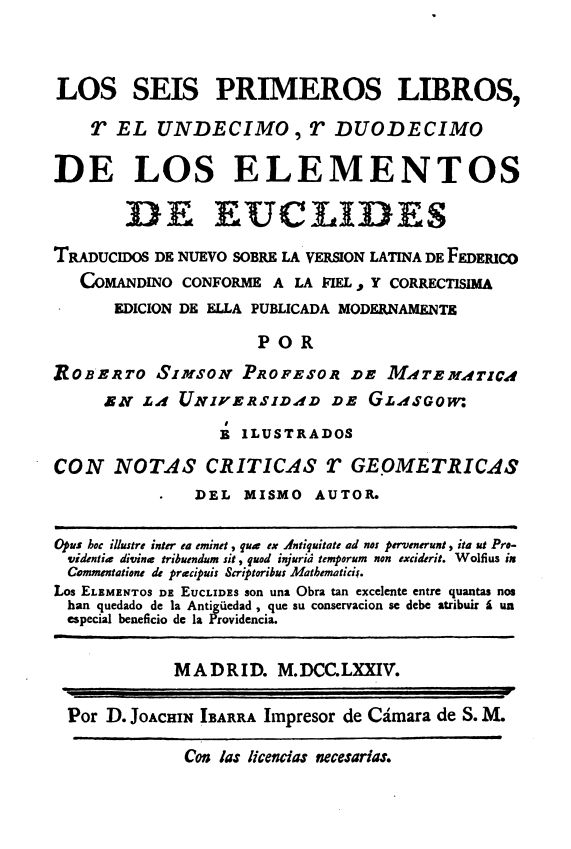
\includegraphics[height=6cm]{./imgs/Euclides_portada.png}}
% \end{frame}

\subsection{Axiomatización de Hilbert}

\begin{frame}[fragile, c]
	\centerline{
		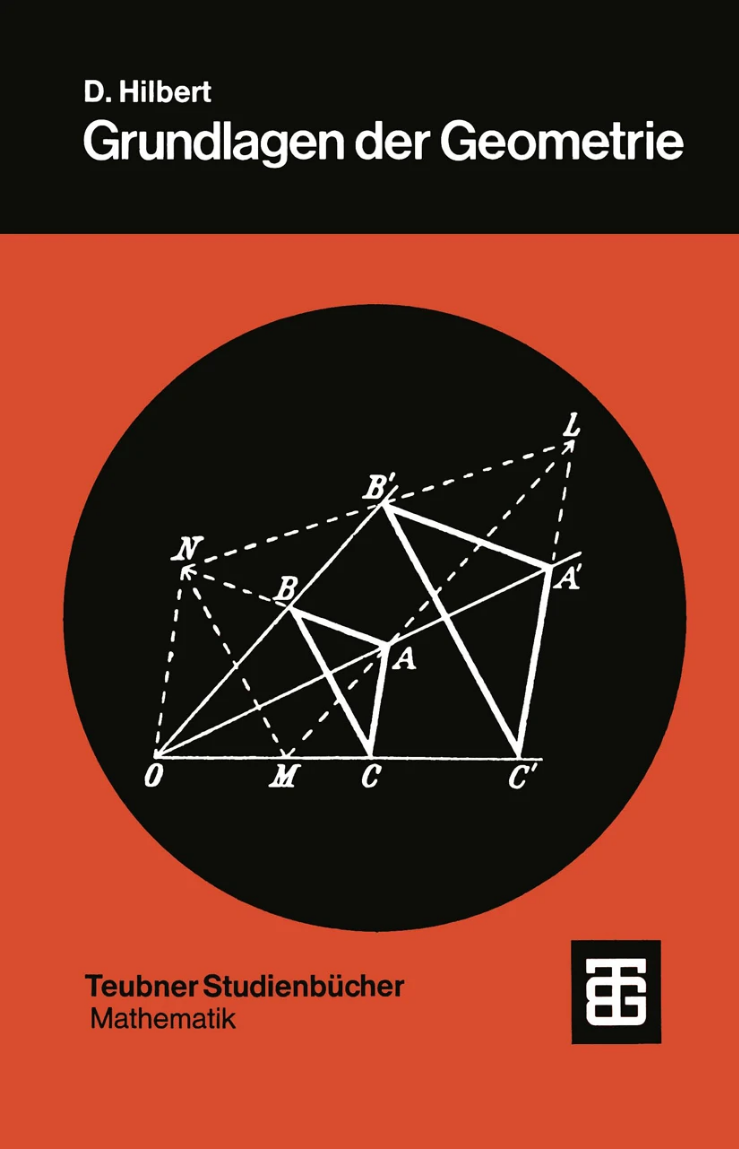
\includegraphics[height=5cm]{./imgs/Hilbert_portada.png}\,
		\pause
		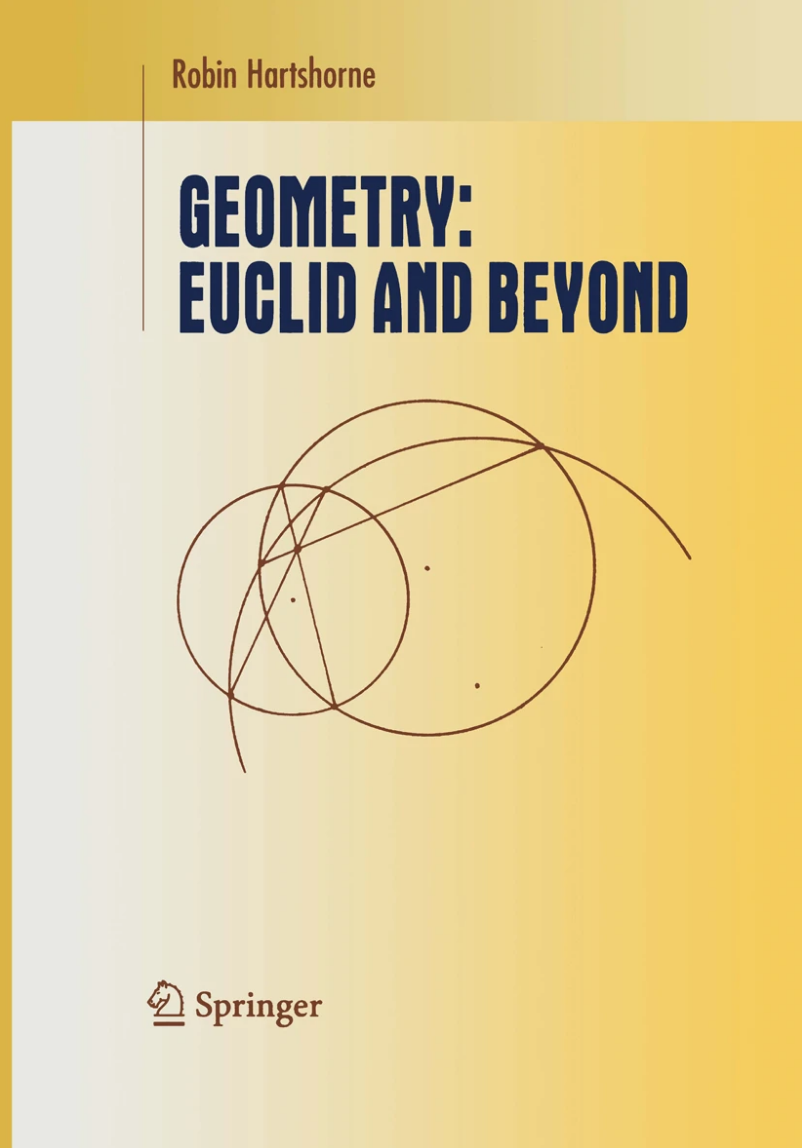
\includegraphics[height=5cm]{./imgs/Hartshorne_portada.png}
		
\includegraphics[height=5cm]{./imgs/Greenberg_portada.png}\,
	}
\end{frame}

% \subsection{Nociones fundamentales}

\begin{frame}[fragile, c]
	\begin{itemize}
		\item \textit{Puntos}. $A, B, C, \dots$
		\item \textit{Líneas}. $l, m, n, \dots$
		\item \textit{incidencia}. $A\sim l$
		\item \textit{orden}. $A * B * C$
		\item \textit{congruencia de segmentos}. $\overline{AB}\cong\overline{CD}$
		\item \textit{congruencia de ángulos}. $\angle ABC \cong\angle CDE$
	\end{itemize}
\end{frame}



\section{Geometría de incidencia}

% \begin{frame}[fragile]
	Relación de \textit{incidencia} entre \textit{puntos} y \textit{líneas}: $A\sim l$

	\pause\vspace{108.5px}

	\begin{lstlisting}
     class incidence_geometry (Point Line : Type*) :=
       (lies_on : Point → Line → Prop)
       (infix ` ~ ` : 50 := lies_on)
    \end{lstlisting}
\end{frame}


\begin{frame}[fragile]
	Relación de \textit{incidencia} entre \textit{puntos} y \textit{líneas}: $A\sim l$
	\begin{block}{Axioma I1}
		Para cada par de puntos distintos $A$ y $B$ existe una única recta que los
		contiene.
	\end{block}

	\vspace{72px}

	\begin{lstlisting}
     class incidence_geometry (Point Line : Type*) :=
       (lies_on : Point → Line → Prop)
       (infix ` ~ ` : 50 := lies_on)|\pause|
       (I1 {A B : Point} (h : A ≠ B) : ∃! l : Line, A ~ l ∧ B ~ l)
    \end{lstlisting}
\end{frame}

\begin{frame}[fragile]
	Relación de \textit{incidencia} entre \textit{puntos} y \textit{líneas}: $A\sim l$
	\begin{block}{Axioma I1}
		Para cada par de puntos distintos $A$ y $B$ existe una única recta que los
		contiene.
	\end{block}

	\begin{block}{Axioma I2}
		Cada línea contiene al menos dos puntos distintos.
	\end{block}

	\vspace{36.5px}

	\begin{lstlisting}
     class incidence_geometry (Point Line : Type*) :=
       (lies_on : Point → Line → Prop)
       (infix ` ~ ` : 50 := lies_on)
       (I1 {A B : Point} (h : A ≠ B) : ∃! l : Line, A ~ l ∧ B ~ l)|\pause|
       (I2 (l : Line) : ∃ A B : Point, A ≠ B ∧ A ~ l ∧ B ~ l)
    \end{lstlisting}
\end{frame}

\begin{frame}[fragile]
	Relación de \textit{incidencia} entre \textit{puntos} y \textit{líneas}: $A\sim l$
	\begin{block}{Axioma I1}
		Para cada par de puntos distintos $A$ y $B$ existe una única recta que los
		contiene.
	\end{block}

	\begin{block}{Axioma I2}
		Cada línea contiene al menos dos puntos distintos.
	\end{block}

	\begin{block}{Axioma I3}
		Existen tres puntos no colineares. Es decir, existen $A$, $B$ y $C$ tales que
		$AB\neq BC$.
	\end{block}

	\begin{lstlisting}
     class incidence_geometry (Point Line : Type*) :=
       (lies_on : Point → Line → Prop)
       (infix ` ~ ` : 50 := lies_on)
       (I1 {A B : Point} (h : A ≠ B) : ∃! l : Line, A ~ l ∧ B ~ l)
       (I2 (l : Line) : ∃ A B : Point, A ≠ B ∧ A ~ l ∧ B ~ l)|\pause|
       (I3 : ∃ A B C : Point, neq3 A B C ∧ ¬ ∃ l : Line,  A ~ l ∧ B ~ l ∧ C ~ l)
    \end{lstlisting}
\end{frame}



\begin{frame}[fragile]
	\begin{lstlisting}
     class incidence_geometry (Point Line : Type*) :=
       (lies_on : Point → Line → Prop)
       (infix ` ~ ` : 50 := lies_on)|\pause|
       (I1 {A B : Point} (h : A ≠ B) : ∃! l : Line, A ~ l ∧ B ~ l)|\pause|
       (I2 (l : Line) : ∃ A B : Point, A ≠ B ∧ A ~ l ∧ B ~ l)|\pause|
       (I3 : ∃ A B C : Point, neq3 A B C ∧ ¬ ∃ l : Line,  A ~ l ∧ B ~ l ∧ C ~ l)
    \end{lstlisting}
\end{frame}

% \begin{frame}[fragile]
	\begin{prop}
		Dos líneas distintas pueden tener como mucho un punto en común.
	\end{prop}
	\vspace{1em}
	\pause

	\begin{lstlisting}
     def is_common_point 
     {Point Line : Type*} [incidence_geometry Point Line] 
     (A : Point) (l m : Line) := 
     A ~ l ∧ A ~ m 
	\end{lstlisting}

	\begin{lstlisting}
     def have_common_point 
     (Point : Type*) {Line : Type*} [incidence_geometry Point Line]
     (l m : Line) := 
     ∃ A : Point, is_common_point A l m
	\end{lstlisting}
\end{frame}










\begin{frame}[fragile]
	\begin{multicols}{2}
		\begin{lstlisting}
lemma neq_lines_have_at_most_one_common_point 
  (Point : Type*) {Line : Type*} 
  [ig : incidence_geometry Point Line] :
  ∀ l m : Line, l ≠ m → 
    (∃! A : Point, is_common_point A l m) 
    ∨ ¬ have_common_point Point l m := 
\end{lstlisting}
		\columnbreak
		\hfill
	\end{multicols}
\end{frame}










\begin{frame}[fragile]
	\begin{multicols}{2}
		\begin{lstlisting}
lemma neq_lines_have_at_most_one_common_point 
  (Point : Type*) {Line : Type*} 
  [ig : incidence_geometry Point Line] :
  ∀ l m : Line, l ≠ m → 
    (∃! A : Point, is_common_point A l m) 
    ∨ ¬ have_common_point Point l m := 
begin
\end{lstlisting}
		\columnbreak
		\begin{lstlisting}

		\end{lstlisting}
	\end{multicols}
\end{frame}










\begin{frame}[fragile]
	\begin{multicols}{2}
		\begin{lstlisting}
lemma neq_lines_have_at_most_one_common_point 
  (Point : Type*) {Line : Type*} 
  [ig : incidence_geometry Point Line] :
  ∀ l m : Line, l ≠ m → 
    (∃! A : Point, is_common_point A l m) 
    ∨ ¬ have_common_point Point l m := 
begin
\end{lstlisting}
		\columnbreak
		\begin{lstlisting}
Point Line: Type u
ig: incidence_geometry Point Line






⊢ ∀ (l m : Line), l ≠ m → 
  (∃! A : Point, is_common_point A l m) 
  ∨ ¬ have_common_point Point l m
		\end{lstlisting}
	\end{multicols}
\end{frame}










\begin{frame}[fragile]
	\begin{multicols}{2}
		\begin{lstlisting}
lemma neq_lines_have_at_most_one_common_point 
  (Point : Type*) {Line : Type*} 
  [ig : incidence_geometry Point Line] :
  ∀ l m : Line, l ≠ m → 
    (∃! A : Point, is_common_point A l m) 
    ∨ ¬ have_common_point Point l m := 
begin
  intros l m
\end{lstlisting}
		\columnbreak
		\begin{lstlisting}
Point Line: Type u
ig: incidence_geometry Point Line






⊢ ∀ (l m : Line), l ≠ m → 
  (∃! A : Point, is_common_point A l m) 
  ∨ ¬ have_common_point Point l m
		\end{lstlisting}
	\end{multicols}
\end{frame}










\begin{frame}[fragile]
	\begin{multicols}{2}
		\begin{lstlisting}
lemma neq_lines_have_at_most_one_common_point 
  (Point : Type*) {Line : Type*} 
  [ig : incidence_geometry Point Line] :
  ∀ l m : Line, l ≠ m → 
    (∃! A : Point, is_common_point A l m) 
    ∨ ¬ have_common_point Point l m := 
begin
  intros l m,
\end{lstlisting}
		\columnbreak
		\begin{lstlisting}
Point Line: Type u
ig: incidence_geometry Point Line
l m : Line





⊢ l ≠ m → 
  (∃! A : Point, is_common_point A l m) 
  ∨ ¬ have_common_point Point l m
		\end{lstlisting}
	\end{multicols}
\end{frame}










\begin{frame}[fragile]
	\begin{multicols}{2}
		\begin{lstlisting}
lemma neq_lines_have_at_most_one_common_point 
  (Point : Type*) {Line : Type*} 
  [ig : incidence_geometry Point Line] :
  ∀ l m : Line, l ≠ m → 
    (∃! A : Point, is_common_point A l m) 
    ∨ ¬ have_common_point Point l m := 
begin
  intros l m,
  contrapose
\end{lstlisting}
		\columnbreak
		\begin{lstlisting}
Point Line: Type u
ig: incidence_geometry Point Line
l m : Line





⊢ l ≠ m → 
  (∃! A : Point, is_common_point A l m) 
  ∨ ¬ have_common_point Point l m
		\end{lstlisting}
	\end{multicols}
\end{frame}










\begin{frame}[fragile]
	\begin{multicols}{2}
		\begin{lstlisting}
lemma neq_lines_have_at_most_one_common_point 
  (Point : Type*) {Line : Type*} 
  [ig : incidence_geometry Point Line] :
  ∀ l m : Line, l ≠ m → 
    (∃! A : Point, is_common_point A l m) 
    ∨ ¬ have_common_point Point l m := 
begin
  intros l m,
  contrapose,
\end{lstlisting}
		\columnbreak
		\begin{lstlisting}
Point Line: Type u
ig: incidence_geometry Point Line
l m : Line





⊢ ¬((∃! A : Point, is_common_point A l m) 
    ∨ ¬ have_common_point Point l m) → 
  ¬ l ≠ m
		\end{lstlisting}
	\end{multicols}
\end{frame}










\begin{frame}[fragile]
	\begin{multicols}{2}
		\begin{lstlisting}
lemma neq_lines_have_at_most_one_common_point 
  (Point : Type*) {Line : Type*} 
  [ig : incidence_geometry Point Line] :
  ∀ l m : Line, l ≠ m → 
    (∃! A : Point, is_common_point A l m) 
    ∨ ¬ have_common_point Point l m := 
begin
  intros l m,
  contrapose,
  push_neg,
  rintro ⟨not_unique, hlm⟩,
  rw exists_unique at not_unique,
  push_neg at not_unique,
  cases hlm with A hA,
  rcases not_unique A hA with ⟨B, ⟨hB, hAB⟩⟩,
  rw ne_comm at hAB,
\end{lstlisting}
		\columnbreak
		\begin{lstlisting}
Point Line: Type u
ig: incidence_geometry Point Line
l m : Line





⊢ ¬((∃! A : Point, is_common_point A l m) 
    ∨ ¬ have_common_point Point l m) → 
  ¬ l ≠ m
\end{lstlisting}
	\end{multicols}
\end{frame}










\begin{frame}[fragile]
	\begin{multicols}{2}
		\begin{lstlisting}
lemma neq_lines_have_at_most_one_common_point 
  (Point : Type*) {Line : Type*} 
  [ig : incidence_geometry Point Line] :
  ∀ l m : Line, l ≠ m → 
    (∃! A : Point, is_common_point A l m) 
    ∨ ¬ have_common_point Point l m := 
begin
  intros l m,
  contrapose,
  push_neg,
  rintro ⟨not_unique, hlm⟩,
  rw exists_unique at not_unique,
  push_neg at not_unique,
  cases hlm with A hA,
  rcases not_unique A hA with ⟨B, ⟨hB, hAB⟩⟩,
  rw ne_comm at hAB,
\end{lstlisting}
		\columnbreak
		\begin{lstlisting}
Point Line: Type u
ig: incidence_geometry Point Line
l m : Line
A B: Point
hA: is_common_point A l m
hB: is_common_point B l m
hAB: A ≠ B

⊢ l = m
\end{lstlisting}
	\end{multicols}
\end{frame}










\begin{frame}[fragile]
	\begin{multicols}{2}
		\begin{lstlisting}
lemma neq_lines_have_at_most_one_common_point 
  (Point : Type*) {Line : Type*} 
  [ig : incidence_geometry Point Line] :
  ∀ l m : Line, l ≠ m → 
    (∃! A : Point, is_common_point A l m) 
    ∨ ¬ have_common_point Point l m := 
begin
  intros l m,
  contrapose,
  push_neg,
  rintro ⟨not_unique, hlm⟩,
  rw exists_unique at not_unique,
  push_neg at not_unique,
  cases hlm with A hA,
  rcases not_unique A hA with ⟨B, ⟨hB, hAB⟩⟩,
  rw ne_comm at hAB,
  exact unique_of_exists_unique (ig.I1 hAB) ⟨hA.1, hB.1⟩ ⟨hA.2, hB.2⟩
\end{lstlisting}
		\columnbreak
		\begin{lstlisting}
Point Line: Type u
ig: incidence_geometry Point Line
l m : Line
A B: Point
hA: is_common_point A l m
hB: is_common_point B l m
hAB: A ≠ B

⊢ l = m
\end{lstlisting}
	\end{multicols}
\end{frame}










% \begin{frame}[fragile]
% 	\begin{multicols}{2}
% 		\begin{lstlisting}
% lemma neq_lines_have_at_most_one_common_point 
%   (Point : Type*) {Line : Type*} 
%   [ig : incidence_geometry Point Line] :
%   ∀ l m : Line, l ≠ m → 
%     (∃! A : Point, is_common_point A l m) 
%     ∨ ¬ have_common_point Point l m := 
% begin
%   intros l m,
%   contrapose,
%   push_neg,
%   rintro ⟨not_unique, hlm⟩,
%   rw exists_unique at not_unique,
%   push_neg at not_unique,
%   cases hlm with A hA,
%   rcases not_unique A hA with ⟨B, ⟨hB, hAB⟩⟩,
%   rw ne_comm at hAB,
%   exact unique_of_exists_unique (ig.I1 hAB) ⟨hA.1, hB.1⟩ ⟨hA.2, hB.2⟩
% \end{lstlisting}
% 		\vspace{1em}
% 		\begin{lstlisting}
% ig.I1 {A B : Point} (h : A ≠ B) : ∃! l : Line, A ~ l ∧ B ~ l
% \end{lstlisting}
% 		\columnbreak
% 		\begin{lstlisting}
% Point Line: Type u
% ig: incidence_geometry Point Line
% l m : Line
% A B: Point
% hA: is_common_point A l m
% hB: is_common_point B l m
% hAB: A ≠ B

% ⊢ l = m
% \end{lstlisting}
% 	\end{multicols}
% \end{frame}










\begin{frame}[fragile]
	\begin{multicols}{2}
		\begin{lstlisting}
lemma neq_lines_have_at_most_one_common_point 
  (Point : Type*) {Line : Type*} 
  [ig : incidence_geometry Point Line] :
  ∀ l m : Line, l ≠ m → 
    (∃! A : Point, is_common_point A l m) 
    ∨ ¬ have_common_point Point l m := 
begin
  intros l m,
  contrapose,
  push_neg,
  rintro ⟨not_unique, hlm⟩,
  rw exists_unique at not_unique,
  push_neg at not_unique,
  cases hlm with A hA,
  rcases not_unique A hA with ⟨B, ⟨hB, hAB⟩⟩,
  rw ne_comm at hAB,
  exact unique_of_exists_unique (ig.I1 hAB) ⟨hA.1, hB.1⟩ ⟨hA.2, hB.2⟩
\end{lstlisting}
		\vspace{1em}
		\begin{lstlisting}
ig.I1 hAB : ∃! l : Line, A ~ l ∧ B ~ l
\end{lstlisting}
		\columnbreak
		\begin{lstlisting}
Point Line: Type u
ig: incidence_geometry Point Line
l m : Line
A B: Point
hA: is_common_point A l m
hB: is_common_point B l m
hAB: A ≠ B

⊢ l = m
\end{lstlisting}
	\end{multicols}
\end{frame}










\begin{frame}[fragile]
	\begin{multicols}{2}
		\begin{lstlisting}
lemma neq_lines_have_at_most_one_common_point 
  (Point : Type*) {Line : Type*} 
  [ig : incidence_geometry Point Line] :
  ∀ l m : Line, l ≠ m → 
    (∃! A : Point, is_common_point A l m) 
    ∨ ¬ have_common_point Point l m := 
begin
  intros l m,
  contrapose,
  push_neg,
  rintro ⟨not_unique, hlm⟩,
  rw exists_unique at not_unique,
  push_neg at not_unique,
  cases hlm with A hA,
  rcases not_unique A hA with ⟨B, ⟨hB, hAB⟩⟩,
  rw ne_comm at hAB,
  exact unique_of_exists_unique (ig.I1 hAB) ⟨hA.1, hB.1⟩ ⟨hA.2, hB.2⟩
end
\end{lstlisting}
		\columnbreak
		\lstinline{goals accomplished} \checkmark
	\end{multicols}
\end{frame}





























\begin{frame}[fragile]
	\begin{prop}
		Dos líneas distintas pueden tener como mucho un punto en común.
	\end{prop}
	\vspace{1em}
	\pause
	\begin{lstlisting}
     def is_common_point (A : Point) (l m : Line) := 
       A ~ l ∧ A ~ m 
	\end{lstlisting}
	\pause
	\begin{lstlisting}
     def have_common_point (l m : Line) := 
       ∃ A : Point, is_common_point A l m
	\end{lstlisting}
\end{frame}










\begin{frame}[fragile]
	\begin{multicols}{2}
		\begin{lstlisting}
lemma neq_lines_have_at_most_one_common_point :
  ∀ l m : Line, l ≠ m → 
    (∃! A : Point, is_common_point A l m) 
    ∨ ¬ have_common_point Point l m := 
\end{lstlisting}
		\columnbreak
		\hfill
	\end{multicols}
\end{frame}










\begin{frame}[fragile]
	\begin{multicols}{2}
		\begin{lstlisting}
lemma neq_lines_have_at_most_one_common_point :
  ∀ l m : Line, l ≠ m → 
    (∃! A : Point, is_common_point A l m) 
    ∨ ¬ have_common_point Point l m := 
begin
\end{lstlisting}
		\columnbreak
		\begin{lstlisting}

		\end{lstlisting}
	\end{multicols}
\end{frame}










\begin{frame}[fragile]
	\begin{multicols}{2}
		\begin{lstlisting}
lemma neq_lines_have_at_most_one_common_point :
  ∀ l m : Line, l ≠ m → 
    (∃! A : Point, is_common_point A l m) 
    ∨ ¬ have_common_point Point l m := 
begin
\end{lstlisting}
		\columnbreak
		\begin{lstlisting}
Point Line: Type u
ig: incidence_geometry Point Line






⊢ ∀ (l m : Line), l ≠ m → 
  (∃! A : Point, is_common_point A l m) 
  ∨ ¬ have_common_point Point l m
		\end{lstlisting}
	\end{multicols}
\end{frame}










\begin{frame}[fragile]
	\begin{multicols}{2}
		\begin{lstlisting}
lemma neq_lines_have_at_most_one_common_point :
  ∀ l m : Line, l ≠ m → 
    (∃! A : Point, is_common_point A l m) 
    ∨ ¬ have_common_point Point l m := 
begin
  intros l m
\end{lstlisting}
		\columnbreak
		\begin{lstlisting}
Point Line: Type u
ig: incidence_geometry Point Line






⊢ ∀ (l m : Line), l ≠ m → 
  (∃! A : Point, is_common_point A l m) 
  ∨ ¬ have_common_point Point l m
		\end{lstlisting}
	\end{multicols}
\end{frame}










\begin{frame}[fragile]
	\begin{multicols}{2}
		\begin{lstlisting}
lemma neq_lines_have_at_most_one_common_point :
  ∀ l m : Line, l ≠ m → 
    (∃! A : Point, is_common_point A l m) 
    ∨ ¬ have_common_point Point l m := 
begin
  intros l m,
\end{lstlisting}
		\columnbreak
		\begin{lstlisting}
Point Line: Type u
ig: incidence_geometry Point Line
l m : Line





⊢ l ≠ m → 
  (∃! A : Point, is_common_point A l m) 
  ∨ ¬ have_common_point Point l m
		\end{lstlisting}
	\end{multicols}
\end{frame}










\begin{frame}[fragile]
	\begin{multicols}{2}
		\begin{lstlisting}
lemma neq_lines_have_at_most_one_common_point :
  ∀ l m : Line, l ≠ m → 
    (∃! A : Point, is_common_point A l m) 
    ∨ ¬ have_common_point Point l m := 
begin
  intros l m,
  contrapose
\end{lstlisting}
		\columnbreak
		\begin{lstlisting}
Point Line: Type u
ig: incidence_geometry Point Line
l m : Line





⊢ l ≠ m → 
  (∃! A : Point, is_common_point A l m) 
  ∨ ¬ have_common_point Point l m
		\end{lstlisting}
	\end{multicols}
\end{frame}










\begin{frame}[fragile]
	\begin{multicols}{2}
		\begin{lstlisting}
lemma neq_lines_have_at_most_one_common_point :
  ∀ l m : Line, l ≠ m → 
    (∃! A : Point, is_common_point A l m) 
    ∨ ¬ have_common_point Point l m := 
begin
  intros l m,
  contrapose,
\end{lstlisting}
		\columnbreak
		\begin{lstlisting}
Point Line: Type u
ig: incidence_geometry Point Line
l m : Line





⊢ ¬((∃! A : Point, is_common_point A l m) 
    ∨ ¬ have_common_point Point l m) → 
  ¬ l ≠ m
		\end{lstlisting}
	\end{multicols}
\end{frame}










\begin{frame}[fragile]
	\begin{multicols}{2}
		\begin{lstlisting}
lemma neq_lines_have_at_most_one_common_point :
  ∀ l m : Line, l ≠ m → 
    (∃! A : Point, is_common_point A l m) 
    ∨ ¬ have_common_point Point l m := 
begin
  intros l m,
  contrapose,
  push_neg
\end{lstlisting}
		\columnbreak
		\begin{lstlisting}
Point Line: Type u
ig: incidence_geometry Point Line
l m : Line





⊢ ¬((∃! A : Point, is_common_point A l m) 
    ∨ ¬ have_common_point Point l m) → 
  ¬ l ≠ m
		\end{lstlisting}
	\end{multicols}
\end{frame}










\begin{frame}[fragile]
	\begin{multicols}{2}
		\begin{lstlisting}
lemma neq_lines_have_at_most_one_common_point :
  ∀ l m : Line, l ≠ m → 
    (∃! A : Point, is_common_point A l m) 
    ∨ ¬ have_common_point Point l m := 
begin
  intros l m,
  contrapose,
  push_neg,
\end{lstlisting}
		\columnbreak
		\begin{lstlisting}
Point Line: Type u
ig: incidence_geometry Point Line
l m : Line





⊢ (¬∃! A : Point, is_common_point A l m) 
   ∧ have_common_point Point l m → 
  l = m
		\end{lstlisting}
	\end{multicols}
\end{frame}










\begin{frame}[fragile]
	\begin{multicols}{2}
		\begin{lstlisting}
lemma neq_lines_have_at_most_one_common_point :
  ∀ l m : Line, l ≠ m → 
    (∃! A : Point, is_common_point A l m) 
    ∨ ¬ have_common_point Point l m := 
begin
  intros l m,
  contrapose,
  push_neg,
  rintro ⟨not_unique, hlm⟩
\end{lstlisting}
		\columnbreak
		\begin{lstlisting}
Point Line: Type u
ig: incidence_geometry Point Line
l m : Line





⊢ (¬∃! A : Point, is_common_point A l m) 
   ∧ have_common_point Point l m → 
  l = m
		\end{lstlisting}
	\end{multicols}
\end{frame}










\begin{frame}[fragile]
	\begin{multicols}{2}
		\begin{lstlisting}
lemma neq_lines_have_at_most_one_common_point :
  ∀ l m : Line, l ≠ m → 
    (∃! A : Point, is_common_point A l m) 
    ∨ ¬ have_common_point Point l m := 
begin
  intros l m,
  contrapose,
  push_neg,
  rintro ⟨not_unique, hlm⟩,
\end{lstlisting}
		\columnbreak
		\begin{lstlisting}
Point Line: Type u
ig: incidence_geometry Point Line
l m : Line
not_unique: ¬∃! A : Point, is_common_point A l m
hlm: have_common_point Point l m



⊢ l = m
		\end{lstlisting}
	\end{multicols}
\end{frame}










\begin{frame}[fragile]
	\begin{multicols}{2}
		\begin{lstlisting}
lemma neq_lines_have_at_most_one_common_point :
  ∀ l m : Line, l ≠ m → 
    (∃! A : Point, is_common_point A l m) 
    ∨ ¬ have_common_point Point l m := 
begin
  intros l m,
  contrapose,
  push_neg,
  rintro ⟨not_unique, hlm⟩,
  rw exists_unique at not_unique
\end{lstlisting}
		\columnbreak
		\begin{lstlisting}
Point Line: Type u
ig: incidence_geometry Point Line
l m : Line
not_unique: ¬∃! A : Point, is_common_point A l m
hlm: have_common_point Point l m



⊢ l = m
		\end{lstlisting}
	\end{multicols}
\end{frame}










\begin{frame}[fragile]
	\begin{multicols}{2}
		\begin{lstlisting}
lemma neq_lines_have_at_most_one_common_point :
  ∀ l m : Line, l ≠ m → 
    (∃! A : Point, is_common_point A l m) 
    ∨ ¬ have_common_point Point l m := 
begin
  intros l m,
  contrapose,
  push_neg,
  rintro ⟨not_unique, hlm⟩,
  rw exists_unique at not_unique,
\end{lstlisting}
		\columnbreak
		\begin{lstlisting}
Point Line: Type u
ig: incidence_geometry Point Line
l m : Line
not_unique: ¬∃ A : Point, 
  is_common_point A l m 
  ∧ ∀ B : Point, is_common_point B l m → B = A
hlm: have_common_point Point l m

⊢ l = m
		\end{lstlisting}
	\end{multicols}
\end{frame}










\begin{frame}[fragile]
	\begin{multicols}{2}
		\begin{lstlisting}
lemma neq_lines_have_at_most_one_common_point :
  ∀ l m : Line, l ≠ m → 
    (∃! A : Point, is_common_point A l m) 
    ∨ ¬ have_common_point Point l m := 
begin
  intros l m,
  contrapose,
  push_neg,
  rintro ⟨not_unique, hlm⟩,
  rw exists_unique at not_unique,
  push_neg at not_unique
\end{lstlisting}
		\columnbreak
		\begin{lstlisting}
Point Line: Type u
ig: incidence_geometry Point Line
l m : Line
not_unique: ¬∃ A : Point, 
  is_common_point A l m 
  ∧ ∀ B : Point, is_common_point B l m → B = A
hlm: have_common_point Point l m

⊢ l = m
		\end{lstlisting}
	\end{multicols}
\end{frame}










\begin{frame}[fragile]
	\begin{multicols}{2}
		\begin{lstlisting}
lemma neq_lines_have_at_most_one_common_point :
  ∀ l m : Line, l ≠ m → 
    (∃! A : Point, is_common_point A l m) 
    ∨ ¬ have_common_point Point l m := 
begin
  intros l m,
  contrapose,
  push_neg,
  rintro ⟨not_unique, hlm⟩,
  rw exists_unique at not_unique,
  push_neg at not_unique,
\end{lstlisting}
		\columnbreak
		\begin{lstlisting}
Point Line: Type u
ig: incidence_geometry Point Line
l m : Line
not_unique: ∀ A : Point, is_common_point A l m → 
  (∃ B : Point, is_common_point B l m ∧ B ≠ A)
hlm: have_common_point Point l m


⊢ l = m
		\end{lstlisting}
	\end{multicols}
\end{frame}










\begin{frame}[fragile]
	\begin{multicols}{2}
		\begin{lstlisting}
lemma neq_lines_have_at_most_one_common_point :
  ∀ l m : Line, l ≠ m → 
    (∃! A : Point, is_common_point A l m) 
    ∨ ¬ have_common_point Point l m := 
begin
  intros l m,
  contrapose,
  push_neg,
  rintro ⟨not_unique, hlm⟩,
  rw exists_unique at not_unique,
  push_neg at not_unique,
  cases hlm with A hA
\end{lstlisting}
		\columnbreak
		\begin{lstlisting}
Point Line: Type u
ig: incidence_geometry Point Line
l m : Line
not_unique: ∀ A : Point, is_common_point A l m → 
  (∃ B : Point, is_common_point B l m ∧ B ≠ A)
hlm: have_common_point Point l m


⊢ l = m
		\end{lstlisting}
	\end{multicols}
\end{frame}










\begin{frame}[fragile]
	\begin{multicols}{2}
		\begin{lstlisting}
lemma neq_lines_have_at_most_one_common_point :
  ∀ l m : Line, l ≠ m → 
    (∃! A : Point, is_common_point A l m) 
    ∨ ¬ have_common_point Point l m := 
begin
  intros l m,
  contrapose,
  push_neg,
  rintro ⟨not_unique, hlm⟩,
  rw exists_unique at not_unique,
  push_neg at not_unique,
  cases hlm with A hA,
\end{lstlisting}
		\columnbreak
		\begin{lstlisting}
Point Line: Type u
ig: incidence_geometry Point Line
l m : Line
not_unique: ∀ A : Point, is_common_point A l m → 
  (∃ B : Point, is_common_point B l m ∧ B ≠ A)
A: Point
hA: is_common_point A l m

⊢ l = m
		\end{lstlisting}
	\end{multicols}
\end{frame}










\begin{frame}[fragile]
	\begin{multicols}{2}
		\begin{lstlisting}
lemma neq_lines_have_at_most_one_common_point :
  ∀ l m : Line, l ≠ m → 
    (∃! A : Point, is_common_point A l m) 
    ∨ ¬ have_common_point Point l m := 
begin
  intros l m,
  contrapose,
  push_neg,
  rintro ⟨not_unique, hlm⟩,
  rw exists_unique at not_unique,
  push_neg at not_unique,
  cases hlm with A hA,
  rcases not_unique A hA with ⟨B, ⟨hB, hAB⟩⟩
\end{lstlisting}
		\columnbreak
		\begin{lstlisting}
Point Line: Type u
ig: incidence_geometry Point Line
l m : Line
not_unique: ∀ A : Point, is_common_point A l m → 
  (∃ B : Point, is_common_point B l m ∧ B ≠ A)
A: Point
hA: is_common_point A l m

⊢ l = m
		\end{lstlisting}
	\end{multicols}
\end{frame}










\begin{frame}[fragile]
	\begin{multicols}{2}
		\begin{lstlisting}
lemma neq_lines_have_at_most_one_common_point :
  ∀ l m : Line, l ≠ m → 
    (∃! A : Point, is_common_point A l m) 
    ∨ ¬ have_common_point Point l m := 
begin
  intros l m,
  contrapose,
  push_neg,
  rintro ⟨not_unique, hlm⟩,
  rw exists_unique at not_unique,
  push_neg at not_unique,
  cases hlm with A hA,
  rcases not_unique A hA with ⟨B, ⟨hB, hAB⟩⟩,
\end{lstlisting}
		\columnbreak
		\begin{lstlisting}
Point Line: Type u
ig: incidence_geometry Point Line
l m : Line
A B: Point
hA: is_common_point A l m
hB: is_common_point B l m
hAB: B ≠ A

⊢ l = m
\end{lstlisting}
	\end{multicols}
\end{frame}










\begin{frame}[fragile]
	\begin{multicols}{2}
		\begin{lstlisting}
lemma neq_lines_have_at_most_one_common_point :
  ∀ l m : Line, l ≠ m → 
    (∃! A : Point, is_common_point A l m) 
    ∨ ¬ have_common_point Point l m := 
begin
  intros l m,
  contrapose,
  push_neg,
  rintro ⟨not_unique, hlm⟩,
  rw exists_unique at not_unique,
  push_neg at not_unique,
  cases hlm with A hA,
  rcases not_unique A hA with ⟨B, ⟨hB, hAB⟩⟩,
  rw ne_comm at hAB
\end{lstlisting}
		\columnbreak
		\begin{lstlisting}
Point Line: Type u
ig: incidence_geometry Point Line
l m : Line
A B: Point
hA: is_common_point A l m
hB: is_common_point B l m
hAB: B ≠ A

⊢ l = m
\end{lstlisting}
	\end{multicols}
\end{frame}










\begin{frame}[fragile]
	\begin{multicols}{2}
		\begin{lstlisting}
lemma neq_lines_have_at_most_one_common_point :
  ∀ l m : Line, l ≠ m → 
    (∃! A : Point, is_common_point A l m) 
    ∨ ¬ have_common_point Point l m := 
begin
  intros l m,
  contrapose,
  push_neg,
  rintro ⟨not_unique, hlm⟩,
  rw exists_unique at not_unique,
  push_neg at not_unique,
  cases hlm with A hA,
  rcases not_unique A hA with ⟨B, ⟨hB, hAB⟩⟩,
  rw ne_comm at hAB,
\end{lstlisting}
		\columnbreak
		\begin{lstlisting}
Point Line: Type u
ig: incidence_geometry Point Line
l m : Line
A B: Point
hA: is_common_point A l m
hB: is_common_point B l m
hAB: A ≠ B

⊢ l = m
\end{lstlisting}
	\end{multicols}
\end{frame}










\begin{frame}[fragile]
	\begin{multicols}{2}
		\begin{lstlisting}
lemma neq_lines_have_at_most_one_common_point :
  ∀ l m : Line, l ≠ m → 
    (∃! A : Point, is_common_point A l m) 
    ∨ ¬ have_common_point Point l m := 
begin
  intros l m,
  contrapose,
  push_neg,
  rintro ⟨not_unique, hlm⟩,
  rw exists_unique at not_unique,
  push_neg at not_unique,
  cases hlm with A hA,
  rcases not_unique A hA with ⟨B, ⟨hB, hAB⟩⟩,
  rw ne_comm at hAB,
  exact unique_of_exists_unique (ig.I1 hAB) ⟨hA.1, hB.1⟩ ⟨hA.2, hB.2⟩
\end{lstlisting}
		\columnbreak
		\begin{lstlisting}
Point Line: Type u
ig: incidence_geometry Point Line
l m : Line
A B: Point
hA: is_common_point A l m
hB: is_common_point B l m
hAB: A ≠ B

⊢ l = m
\end{lstlisting}
	\end{multicols}
\end{frame}










% \begin{frame}[fragile]
% 	\begin{multicols}{2}
% 		\begin{lstlisting}
% lemma neq_lines_have_at_most_one_common_point :
%   (Point : Type*) {Line : Type*} 
%   [ig : incidence_geometry Point Line] :
%   ∀ l m : Line, l ≠ m → 
%     (∃! A : Point, is_common_point A l m) 
%     ∨ ¬ have_common_point Point l m := 
% begin
%   intros l m,
%   contrapose,
%   push_neg,
%   rintro ⟨not_unique, hlm⟩,
%   rw exists_unique at not_unique,
%   push_neg at not_unique,
%   cases hlm with A hA,
%   rcases not_unique A hA with ⟨B, ⟨hB, hAB⟩⟩,
%   rw ne_comm at hAB,
%   exact unique_of_exists_unique (ig.I1 hAB) ⟨hA.1, hB.1⟩ ⟨hA.2, hB.2⟩
% \end{lstlisting}
% 		\vspace{1em}
% 		\begin{lstlisting}
% ig.I1 {A B : Point} (h : A ≠ B) : ∃! l : Line, A ~ l ∧ B ~ l
% \end{lstlisting}
% 		\columnbreak
% 		\begin{lstlisting}
% Point Line: Type u
% ig: incidence_geometry Point Line
% l m : Line
% A B: Point
% hA: is_common_point A l m
% hB: is_common_point B l m
% hAB: A ≠ B

% ⊢ l = m
% \end{lstlisting}
% 	\end{multicols}
% \end{frame}










\begin{frame}[fragile]
	\begin{multicols}{2}
		\begin{lstlisting}
lemma neq_lines_have_at_most_one_common_point :
  ∀ l m : Line, l ≠ m → 
    (∃! A : Point, is_common_point A l m) 
    ∨ ¬ have_common_point Point l m := 
begin
  intros l m,
  contrapose,
  push_neg,
  rintro ⟨not_unique, hlm⟩,
  rw exists_unique at not_unique,
  push_neg at not_unique,
  cases hlm with A hA,
  rcases not_unique A hA with ⟨B, ⟨hB, hAB⟩⟩,
  rw ne_comm at hAB,
  exact unique_of_exists_unique (ig.I1 hAB) ⟨hA.1, hB.1⟩ ⟨hA.2, hB.2⟩
\end{lstlisting}
		\vspace{1em}
		\begin{lstlisting}
ig.I1 hAB : ∃! l : Line, A ~ l ∧ B ~ l
\end{lstlisting}
		\columnbreak
		\begin{lstlisting}
Point Line: Type u
ig: incidence_geometry Point Line
l m : Line
A B: Point
hA: is_common_point A l m
hB: is_common_point B l m
hAB: A ≠ B

⊢ l = m
\end{lstlisting}
	\end{multicols}
\end{frame}










\begin{frame}[fragile]
	\begin{multicols}{2}
		\begin{lstlisting}
lemma neq_lines_have_at_most_one_common_point :
  ∀ l m : Line, l ≠ m → 
    (∃! A : Point, is_common_point A l m) 
    ∨ ¬ have_common_point Point l m := 
begin
  intros l m,
  contrapose,
  push_neg,
  rintro ⟨not_unique, hlm⟩,
  rw exists_unique at not_unique,
  push_neg at not_unique,
  cases hlm with A hA,
  rcases not_unique A hA with ⟨B, ⟨hB, hAB⟩⟩,
  rw ne_comm at hAB,
  exact unique_of_exists_unique (ig.I1 hAB) ⟨hA.1, hB.1⟩ ⟨hA.2, hB.2⟩
end
\end{lstlisting}
		\columnbreak
		\lstinline{goals accomplished} \checkmark
	\end{multicols}
\end{frame}































\section{Geometría del orden}

\begin{frame}[fragile]
	\begin{defin*}
		Dados dos puntos distintos $A, B$ el \textbf{segmento}
		$\overline{AB}$ es el \textit{conjunto de puntos} que contiene a $A, B$ y a todos los
		puntos que están entre ellos.
	\end{defin*}
\end{frame}

\begin{frame}[fragile]
	\begin{defin*}
		Dos puntos distintos $A, B$ determinan el \textbf{segmento} $\overline{AB}$.
	\end{defin*}
	\begin{lstlisting}
     structure Seg (Point : Type*) := {A B : Point} (neq : A ≠ B)
    \end{lstlisting}

	\pause

	\begin{defin*}
		Un punto $C$ \textbf{pertenece} al segmento $\overline{AB}$
		si coincide con $A$ o $B$ o está entre ellos ($A * C * B$).
	\end{defin*}
	\begin{lstlisting}
     def Seg.in (seg : Seg Point) (Line : Type*) 
       [og : order_geometry Point Line]  (P : Point) : Prop := 
       P = seg.A ∨ P = seg.B ∨ (og.between seg.A P seg.B)
    \end{lstlisting}
\end{frame}

\begin{frame}[fragile]

	\setcounter{tma}{2}
	\begin{tma}
		Dados dos puntos distintos $A$ y $C$ existe un tercer punto $B$ que se
		encuentra entre ellos: $A * B * C$.
	\end{tma}
	\vspace{1em}\pause
	\centerline{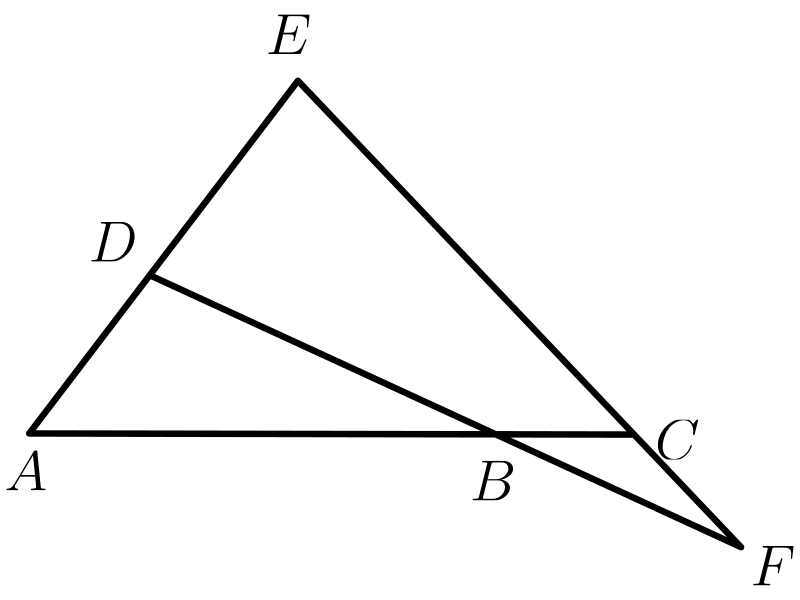
\includegraphics[width=4cm]{./imgs/teorema3.png}}\\
	\vspace{1em}
	\textit{Formalizing Hilbert’s Grundlagen in Isabelle/Isar},\\
	Laura I. Meikle and Jacques D. Fleuriot.\\
\end{frame}

\section{Independencia del axioma de las paralelas}
\begin{frame}[fragile]
	\begin{lstlisting}
     def parallel (Point : Type*) {Line : Type*} [ig : incidence_geometry Point Line] 
       (l m : Line) : Prop := ¬ ∃ P : Point, is_common_point P l m
     |\pause|
     def P (Point Line : Type*) [ig : incidence_geometry Point Line] := 
       ∀ (l : Line) (A : Point), ¬ A ~ l → ∃! m : Line, A ~ m ∧ parallel Point l m
    \end{lstlisting}
	\pause
	\begin{multicols}{2}
		\begin{lstlisting}
     theorem parallels_independence :
       ¬ ∀ plane : hilbert_plane Point Line, 
           P Point Line := 
     begin
       sorry
     end
        \end{lstlisting}
		\columnbreak
		\pause
		\begin{lstlisting}
Point: Type u_1
Line: Type u_2
⊢ ¬ ∀ plane : hilbert_plane Point Line, 
      P Point Line
        \end{lstlisting}
	\end{multicols}
\end{frame}

\begin{frame}[fragile]
	\begin{lstlisting}
     def parallel (Point : Type*) {Line : Type*} [ig : incidence_geometry Point Line] 
       (l m : Line) : Prop := ¬ ∃ P : Point, is_common_point P l m

     def P (Point Line : Type*) [ig : incidence_geometry Point Line] := 
       ∀ (l : Line) (A : Point), ¬ A ~ l → ∃! m : Line, A ~ m ∧ parallel Point l m
    \end{lstlisting}

	\begin{multicols}{2}
		\begin{lstlisting}
     theorem parallels_independence :
       ¬ ∀ plane : hilbert_plane Point Line, 
           P Point Line := 
     begin
       push_neg, 
       sorry
     end
        \end{lstlisting}
		\columnbreak

		\begin{lstlisting}
Point: Type u_1
Line: Type u_2
⊢ ∃ plane : hilbert_plane Point Line, 
      ¬ P Point Line
        \end{lstlisting}
	\end{multicols}
\end{frame}

\section{Conclusiones}

\begin{frame}[fragile, c]
	\begin{itemize}[<+->]
		\item Cumplimiento del proyecto de formalización de Hilbert.
		\item Lean como herramienta de estudio.
		\item Dificultades con \textit{mathlib}, en particular al intentar
		      definir modelos.
		\item Queda mucha geometría por formalizar en Lean.
	\end{itemize}
\end{frame}

\section{¡Gracias!}

\begin{frame}[c]
	\vspace{7px}
	\begin{figure}
		\includegraphics[height=180px]{./imgs/Scuola_di_Atene_Raffaello.png}
		\caption*{\scriptsize
			Detalle de \textit{La escuela de Atenas}, de Rafael Sanzio, \\
			donde vemos a Euclides enseñando a sus alumnos.
		}
	\end{figure}
\end{frame}

\end{document}































